%!TEX root = ../main.tex

\section{Evaluation}
We have implemented our hybrid rule learning approach in Java within a system prototype RuLES,
and conducted experiments on a Linux machine with 80 cores and 500GB RAM.
In this section we report the results of our experimental evaluation, which focuses on 
\emph{(i)} the benefits of our hybrid embedding-based rule quality measure over traditional rule measures; 
\emph{(ii)} the effectiveness of RuLES against the state-of-art Horn rule learning systems; and 
\emph{(iii)} the quality of non-monotonic rules learned by RuLES compared to existing methods.

\subsection{Experimental Setup}
\label{sec:exper_setup}

\subsubsection{Datasets.}
We performed experiments on the following two real world datasets: 
\begin{itemize}
\item \textit{FB15K}~\cite{Bordes:NIPS2013}: a subset of Freebase with 592K binary facts over 15K entities and 1345 relations
commonly used for evaluating KG embedding models~\cite{DBLP:journals/tkde/WangMWG17}.
\item \textit{Wiki44K}: a dataset with 250K binary facts over 44K entities and 100 relations, which is a subset of 
Wikidata dataset from December 2014
used in~\cite{amie}.
\end{itemize}

In the experiments for each incomplete KG $\G$ we need its \emph{ideal} completion $\G^i$ that would give us a gold standard for evaluating our approach and comparing it to others.
Since obtaining a real life $\G^i$ is hard, we used the KGs FB15K 
and Wiki44K as reference graphs $\cG^i_{appr}$ that approximate $\cG^i$. 
We then constructed $\G$ by randomly selecting $80\%$ of its facts while preserving the distribution of facts over predicates.

\subsubsection{Embedding models.}
We experimented with the three state-of-the-art embedding models:
TransE \cite{Bordes:NIPS2013}, HolE \cite{DBLP:conf/aaai/NickelRP16}, and the text-enhanced SSP \cite{DBLP:conf/aaai/0005HMZ17} model. We reuse the implementation of TransE, HolE\footnote{https://github.com/mnick/scikit-kge}, and SSP\footnote{https://github.com/bookmanhan/Embedding}.
TransE and HolE were trained on $\cG$ and SSP on $\cG$ enriched with 
a textual description for each entity extracted from Wikidata. We compared the
effectiveness of the models and selected for every KG the best one. Apart from SSP, which showed the best performance on both KGs, we also selected HolE for FB15K and TransE for Wiki44K. Note that in this work as a proof of concept we considered some of the most popular embedding models, but conceptually any model (see \cite{DBLP:journals/tkde/WangMWG17} for overview) can be used in our system.


\subsubsection{Evaluation metric.} 
To evaluate the learned rules we use the quality of predictions that they produce 
when applied on $\cG$, i.e., the more correct facts beyond $\cG$ a ruleset produces, the better it is.  
We consider two evaluation settings: \emph{closed world} setting (CW) and \emph{open world} setting (OW). 
In the CW setting, we define the prediction precision of a rule $r$ and a set of rules $R$ as:
\begin{align*}
  pred\_prec_{CW}(r) = \frac{|\cG_r \cap \cG^i_{appr} \setminus \cG|}{|\cG_r \setminus \cG|},
  \quad 
  pred\_prec_{CW}(R) = \frac{\sum\limits_{r\in R} pred\_prec_{CW}(r)}{|R|}.
\end{align*}  
In the OW setting, we also take into account the incompleteness of $\cG^i_{\mi{appr}}$ and  
consider the quality of predictions outside it by performing a random sampling and manually annotating the sampled facts relying on Web resources such as Wikipedia. Thus, we define the OW prediction precision $\mi{pred\_prec_{OW}}$ for a set of rules $R$ as follows:
\[
pred\_prec_{OW}(R) = \frac{|\cG'\cap \cG^i_{\mi{appr}}|+|\cG'\backslash \cG^i_{\mi{appr}}|\times \mi{accuracy(\cG'\backslash \cG^i_{\mi{appr}})}}{|\cG'|}.
\]
where $\cG'=\bigcup_{r\in R}\cG_r\backslash \cG$ is the union of predictions generated by rules in $R$, and $\mi{accuracy(S)}$ is the approximated ratio of true facts inside $S$ computed via manual checking of facts sampled from $S$.
Finally, to evaluate the meaningfulness of exceptions in a rule (i.e., negated atoms) we compute the \textit{revision precision}, which according to~\cite{trantowards} is defined as the ratio of incorrect facts in the difference between predictions produced by the Horn part of a rule and its non-monotonic version over the total number of predictions in this difference (the higher the revision precision, the better the rule exceptions) computed per ruleset. Formally,
\begin{align*}
rev\_prec_{OW}(R) = 1-\frac{|\cG'' \cap \cG^i_{\mi{appr}}|+|\cG''\backslash \cG^i_{\mi{appr}}|\times \mi{accuracy(\cG''\backslash \cG^i_{\mi{appr}})}}{|\cG''|}.
\end{align*}
where $\cG''=\cG_H\backslash \cG_R$ and $H$ is the set of Horn parts of rules in $R$. 
Intuitively, $\G''$ contains facts not predicted by the rules in $R$ but predicted by their Horn versions. 
 
\subsubsection{RuLES configuration.} 
We run RuLES in several configurations where $\mu_1$ is set to either \textit{standard confidence (Conf)} or \textit{PCA confidence (PCA)}, and $\mu_2$ is computed based on either TransE, HolE, or SSP models.
Through the experiments the configurations are named as \textbf{$\mu_1$-$\mu_2$} (e.g. Conf-HolE).


\subsection{Embedding-Based Hybrid Quality Function}
\captionsetup[subfigure]{textfont=scriptsize}
 \begin{figure}[t]
     \centering
      %Gad: to unify legend and save space
     \subfloat{{
\includegraphics[width=0.6\textwidth]{figures/new_exp1/legend-crop.pdf} }}\\[-1ex]
     \setcounter{subfigure}{0}
     \subfloat[Conf-HolE on FB15K]{{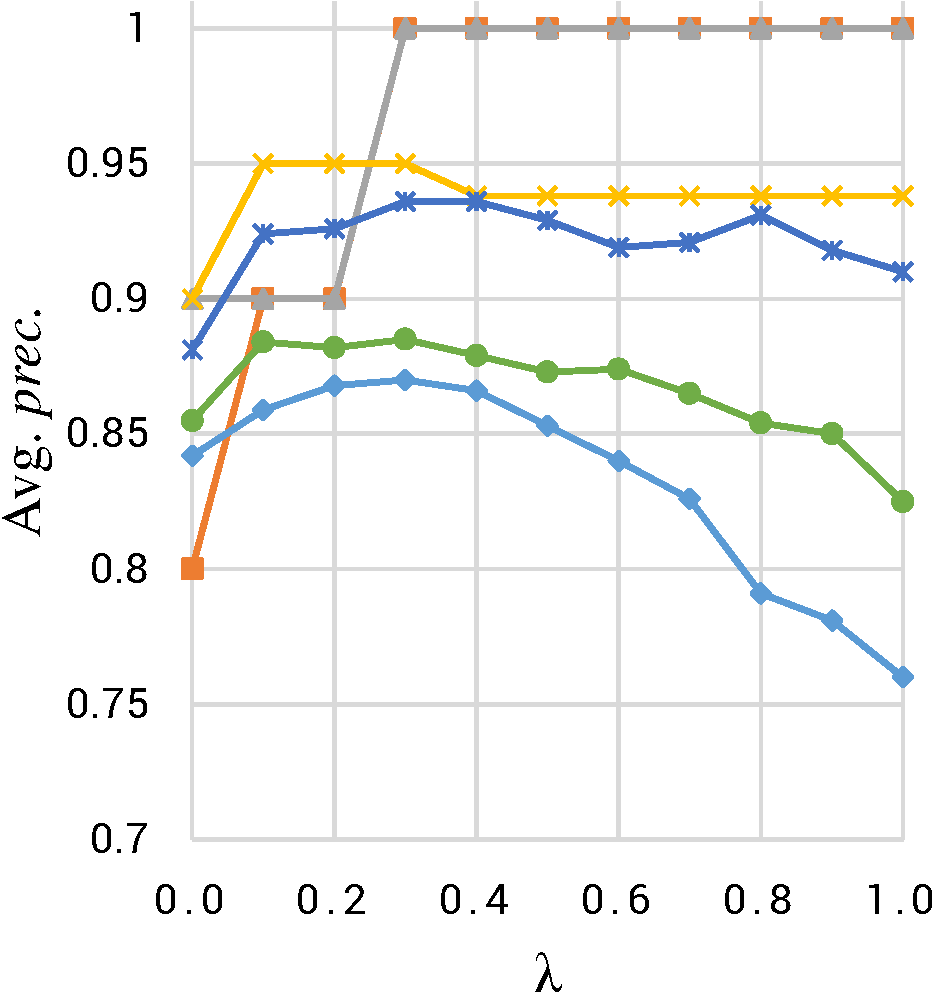
\includegraphics[width=0.3\textwidth]{figures/new_exp1/fb15k_hole_conf-crop.pdf} }\label{fig:fb-HoLE-Conf}}
     \subfloat[Conf-SSP on FB15K]{{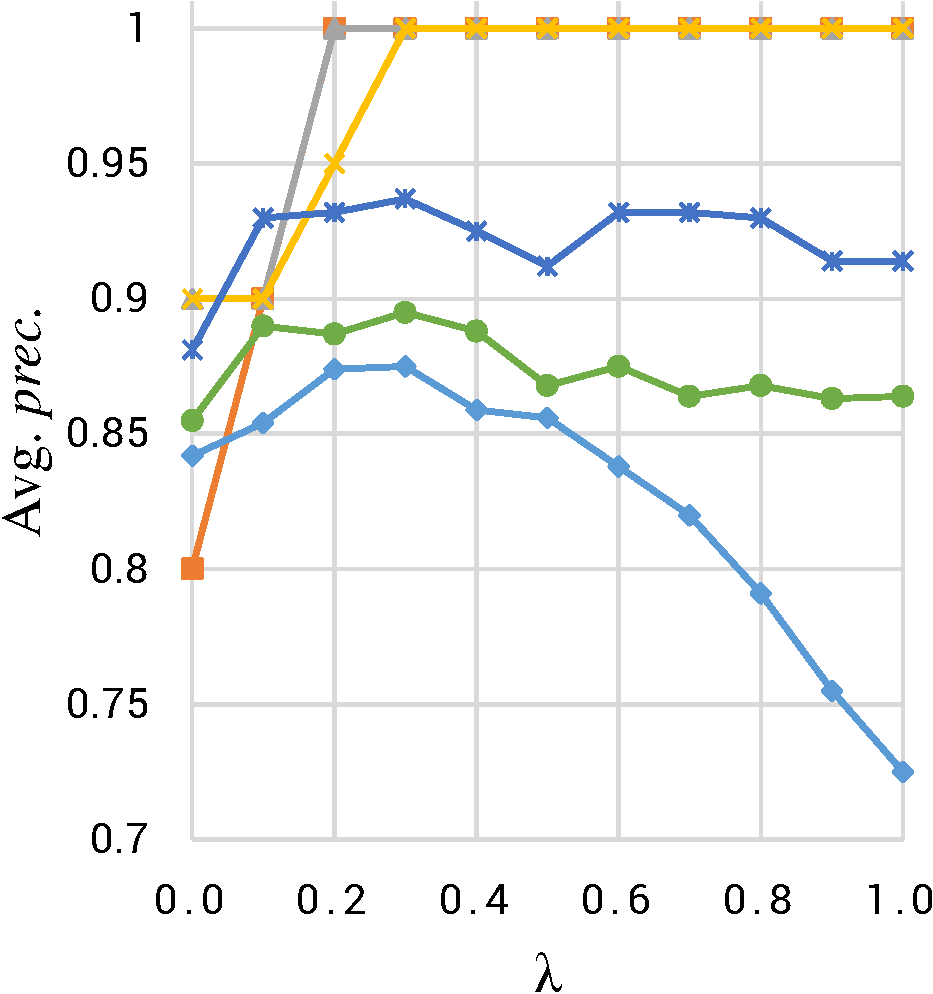
\includegraphics[width=0.3\textwidth]{figures/new_exp1/fb15k_ssp_conf-crop.pdf} \label{fig:fb-SSP-Conf}}}
     %\subfloat[RulES-H-PCA on FB15K]{{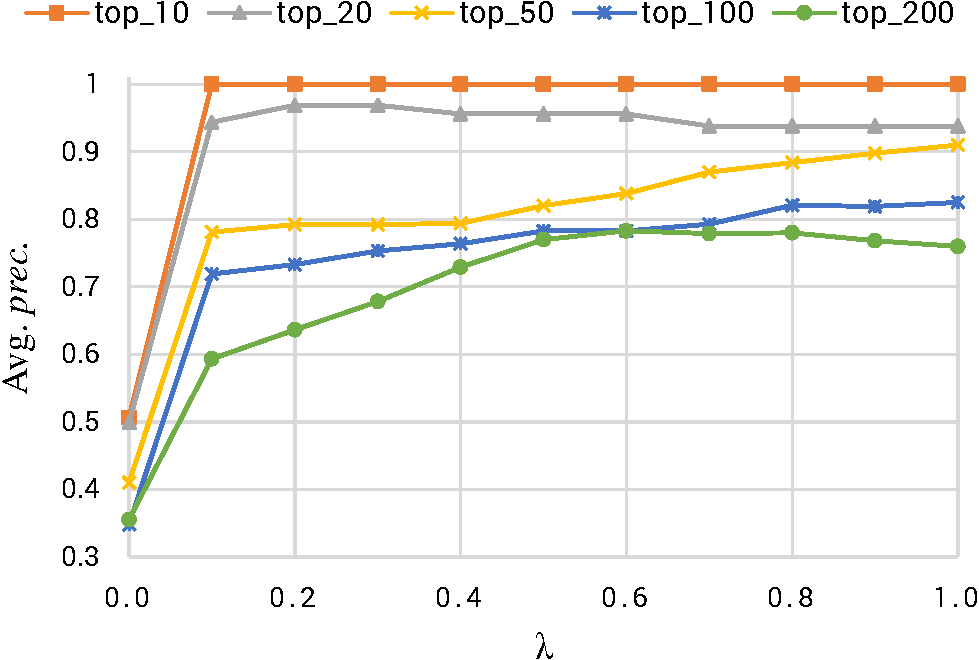
\includegraphics[width=0.3\textwidth]{figures/fb15k_hole_pca-crop.pdf} }}
    \subfloat[PCA-SSP on FB15K]{{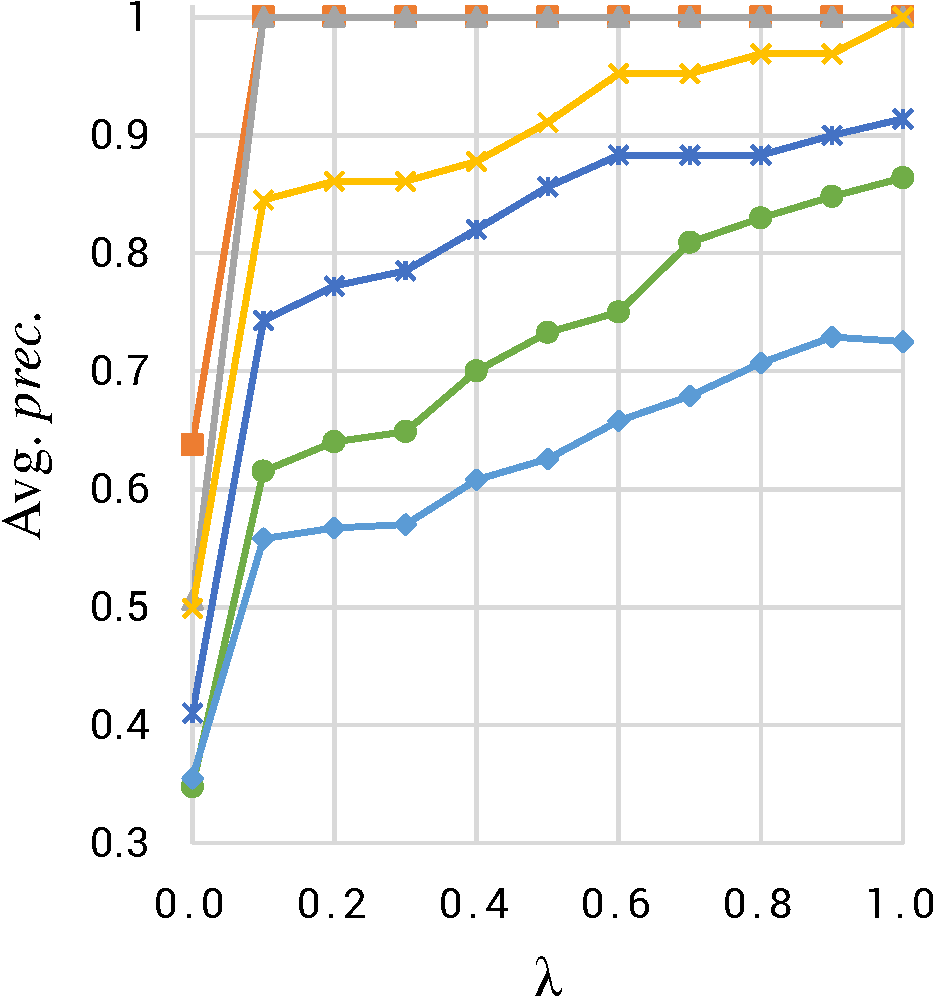
\includegraphics[width=0.3\textwidth]{figures/new_exp1/fb15k_ssp_pca-crop.pdf} }\label{fig:fb-SSP-PCA}} \\   
    
    \subfloat[Conf-TransE on Wiki44K]{{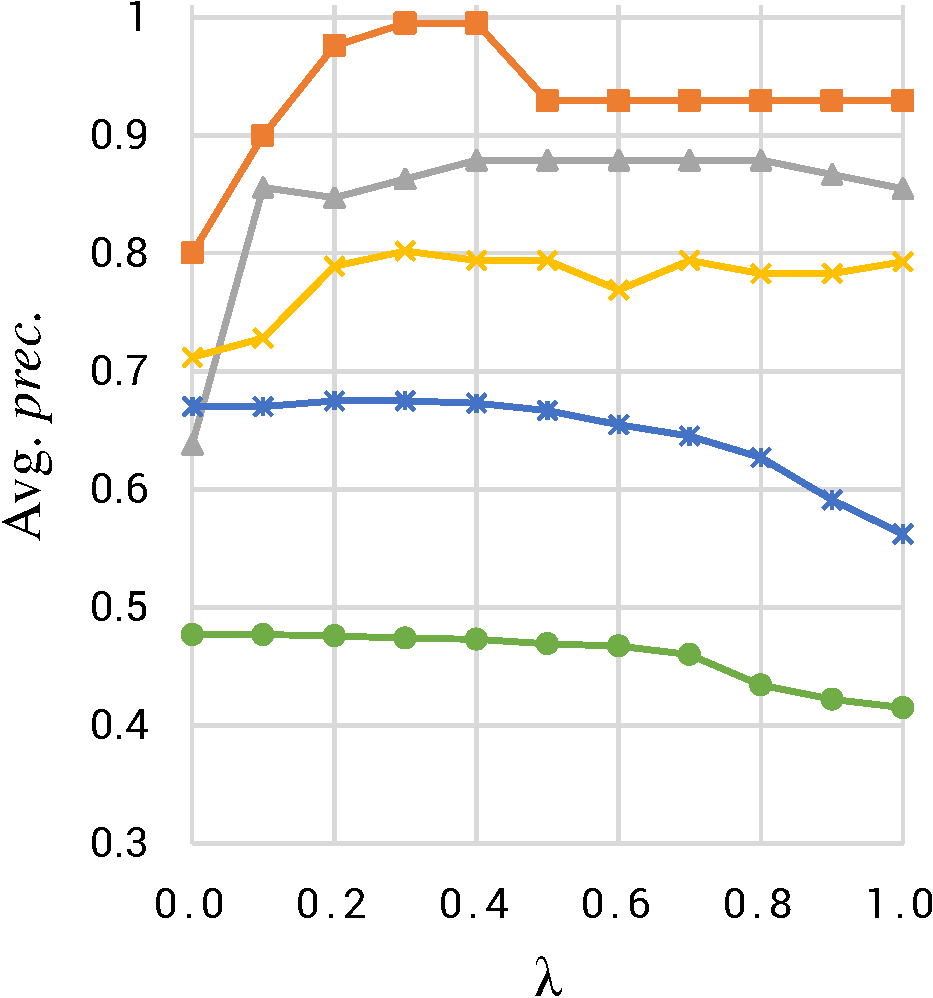
\includegraphics[width=0.3\textwidth]{figures/new_exp1/wiki44k_transe_conf-crop.pdf} }\label{fig:wi-TransE-Conf}}
    \subfloat[Conf-SSP on Wiki44K]{{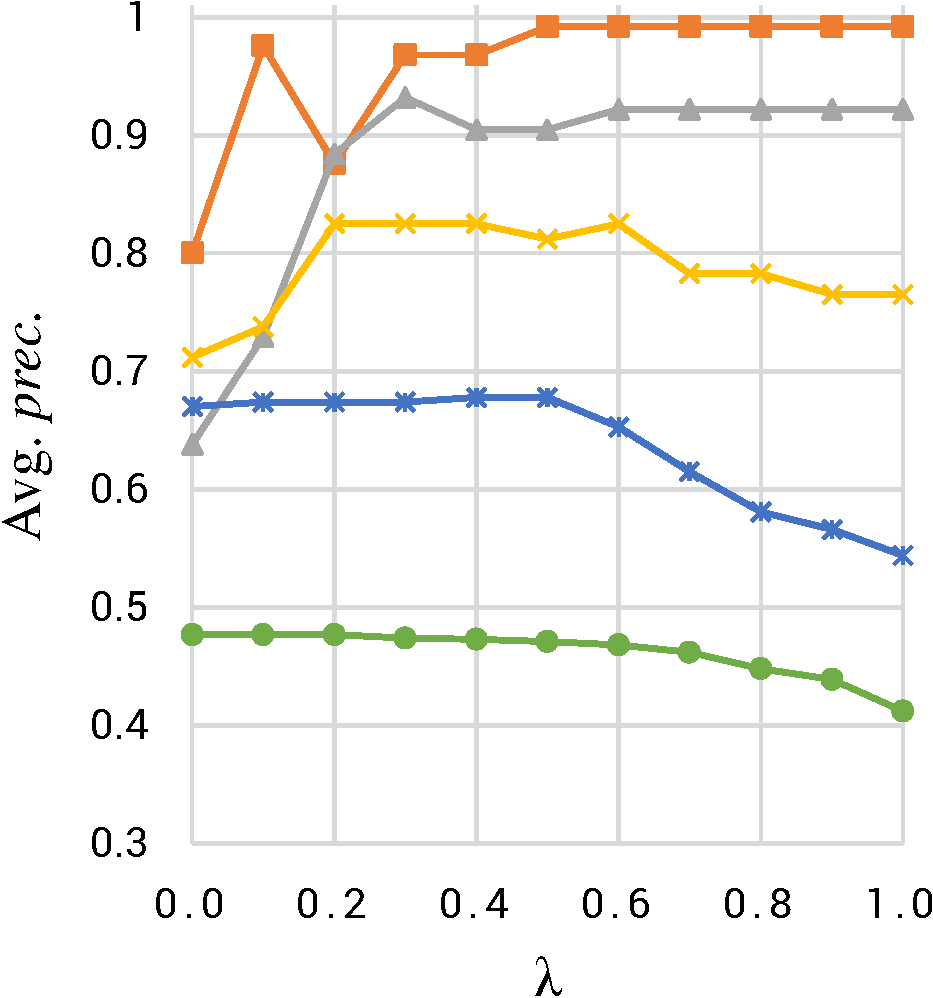
\includegraphics[width=0.3\textwidth]{figures/new_exp1/wiki44k_ssp_conf-crop.pdf} }\label{fig:wi-SSP-Conf}}
     %\subfloat[RulES-H-PCA on Wiki44K]{{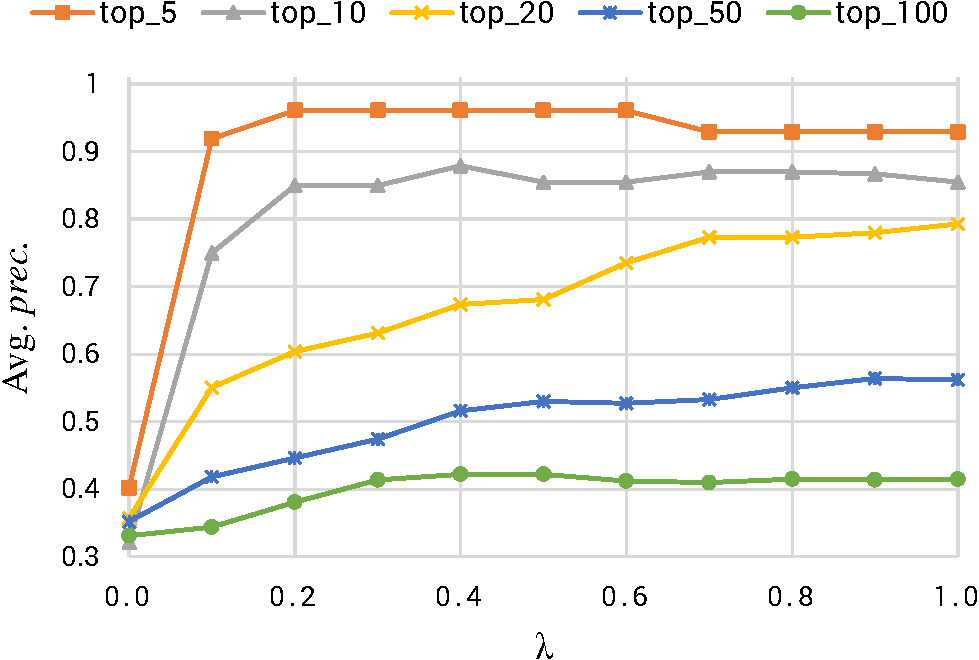
\includegraphics[width=0.3\textwidth]{figures/wiki44k_transe_pca-crop.pdf} }}
     \subfloat[PCA-SSP on Wiki44K]{{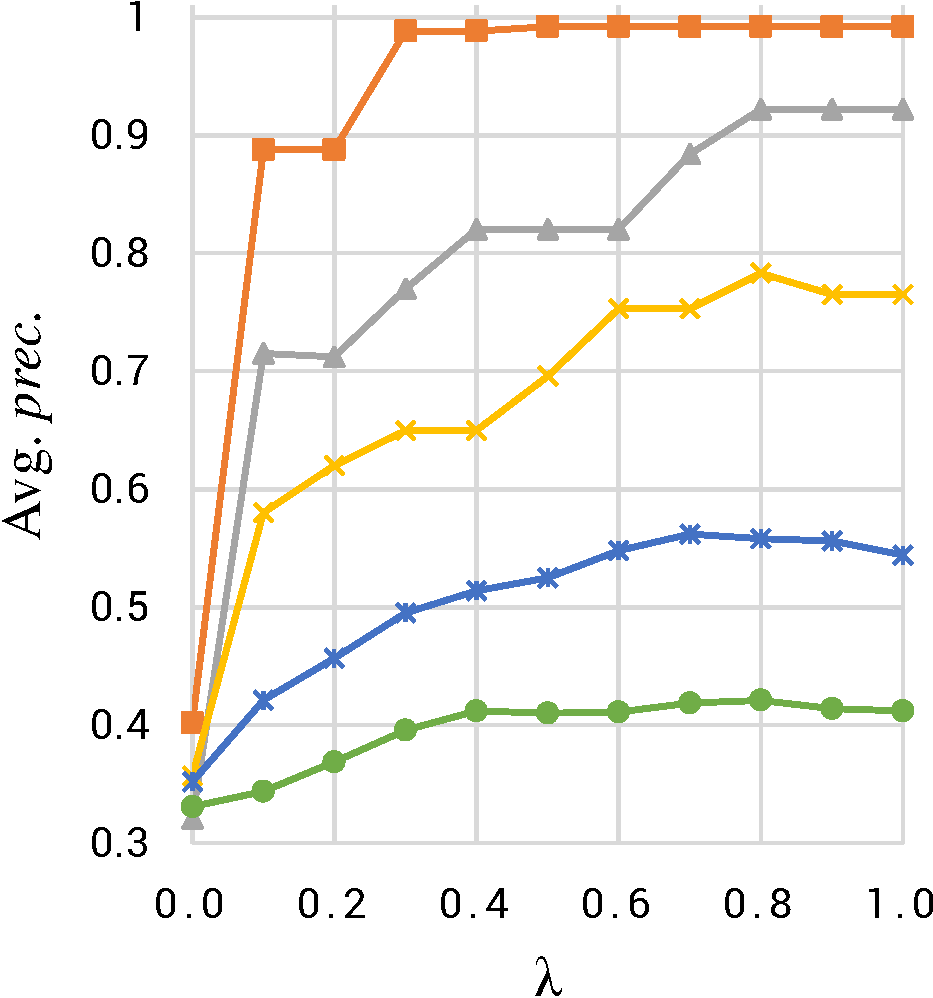
\includegraphics[width=0.3\textwidth]{figures/new_exp1/wiki44k_ssp_pca-crop.pdf} }\label{fig:wi-SSP-PCA}} \\  
    
     \caption{$pred\_prec_{CW}$ of the \textit{top-k} rules with various \textit{embedding weights}.}
     \label{fig:diff_lambda}
 \end{figure}
%\captionsetup[subfigure]{labelformat=empty}
%\begin{figure}[t]
%    \centering    
%    % \vspace*{-3mm}
%    \subfloat{{
\includegraphics[width=0.5\textwidth]{figures/new_exp1/legend-crop.pdf} }}\\[-2ex]
%    \subfloat[FB15K(conf + HolE)]{{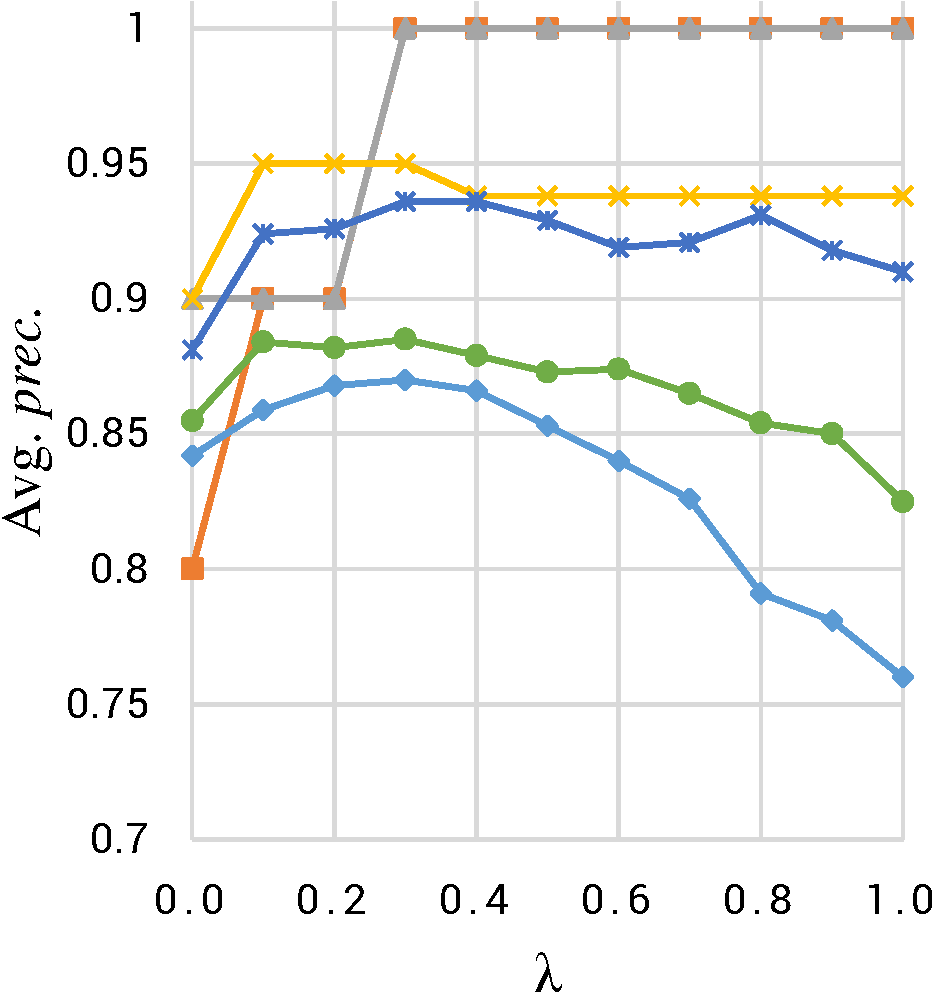
\includegraphics[width=0.33\textwidth]{figures/new_exp1/fb15k_hole_conf-crop.pdf} }}
%    \subfloat[FB15K(conf + SSP)]{{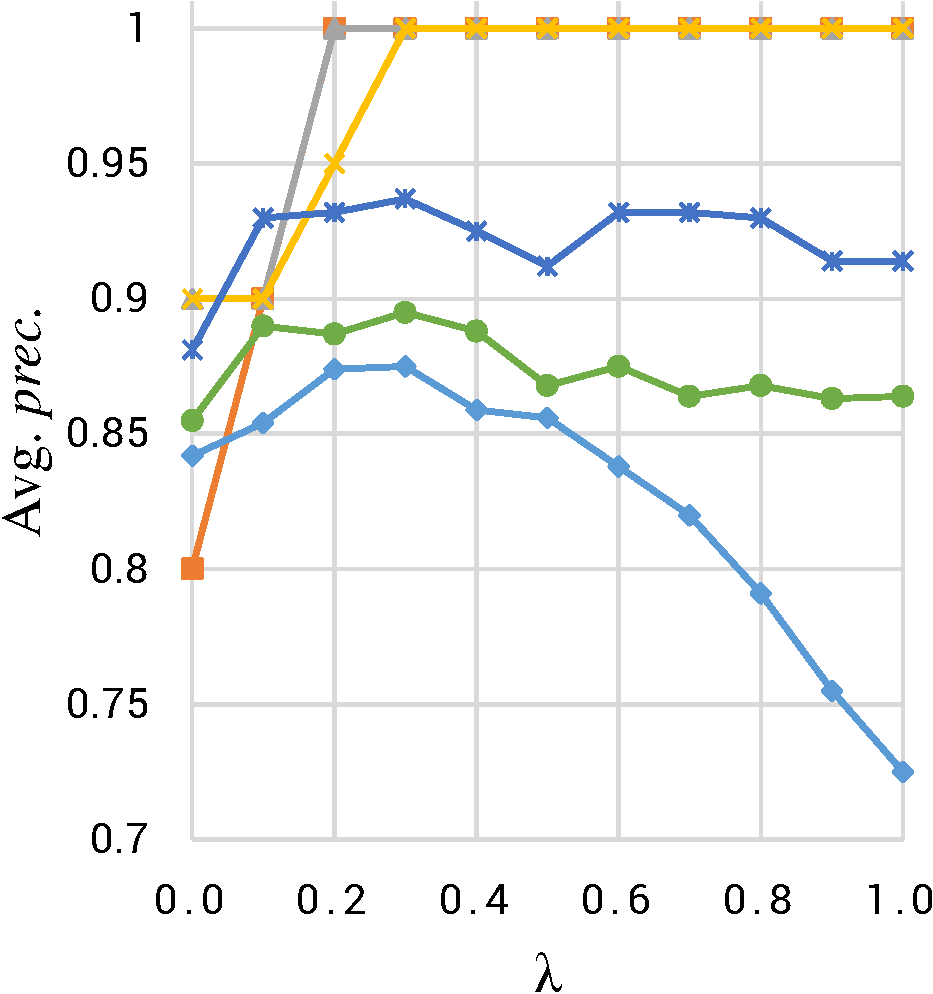
\includegraphics[width=0.33\textwidth]{figures/new_exp1/fb15k_ssp_conf-crop.pdf} }}
%    % \subfloat[PCA Confidence + HolE]{{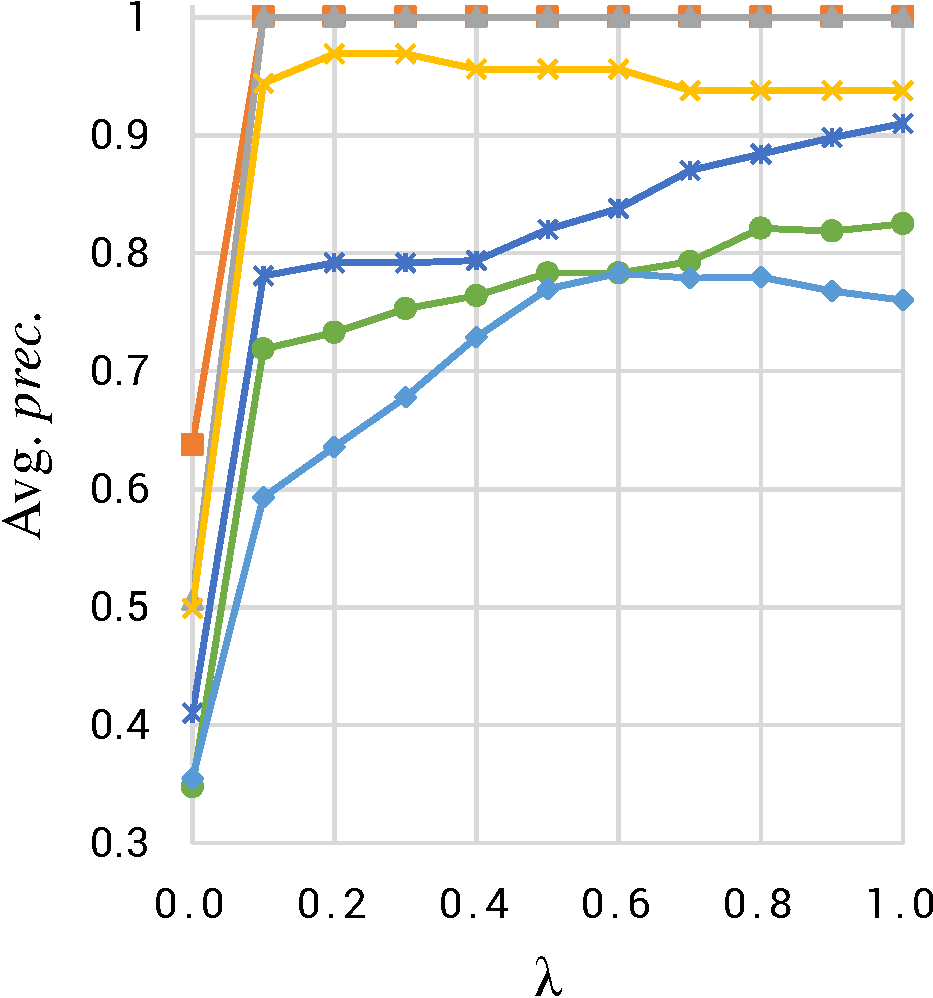
\includegraphics[width=0.5\textwidth]{figures/new_exp1/fb15k_hole_pca-crop.pdf} }}
%    \subfloat[FB15K(pcaconf + SSP)]{{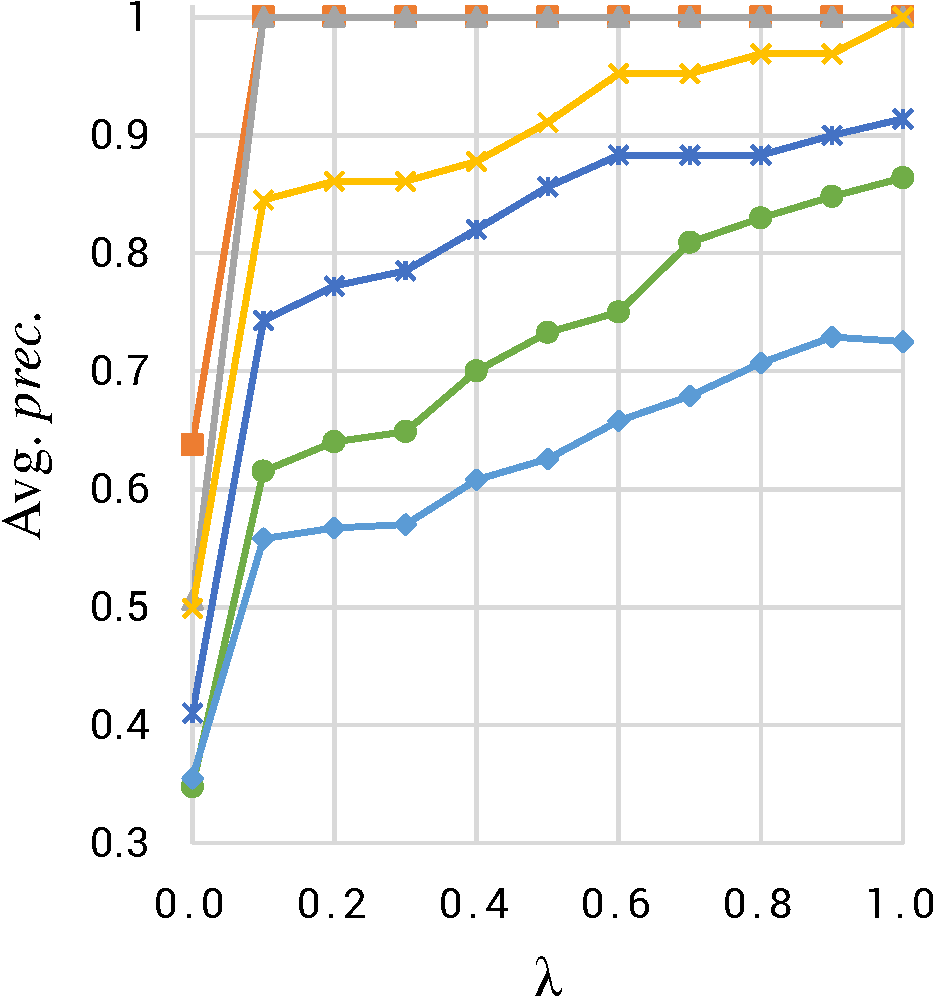
\includegraphics[width=0.33\textwidth]{figures/new_exp1/fb15k_ssp_pca-crop.pdf} }}\\
%    \subfloat[Wiki44K(conf + TransE)]{{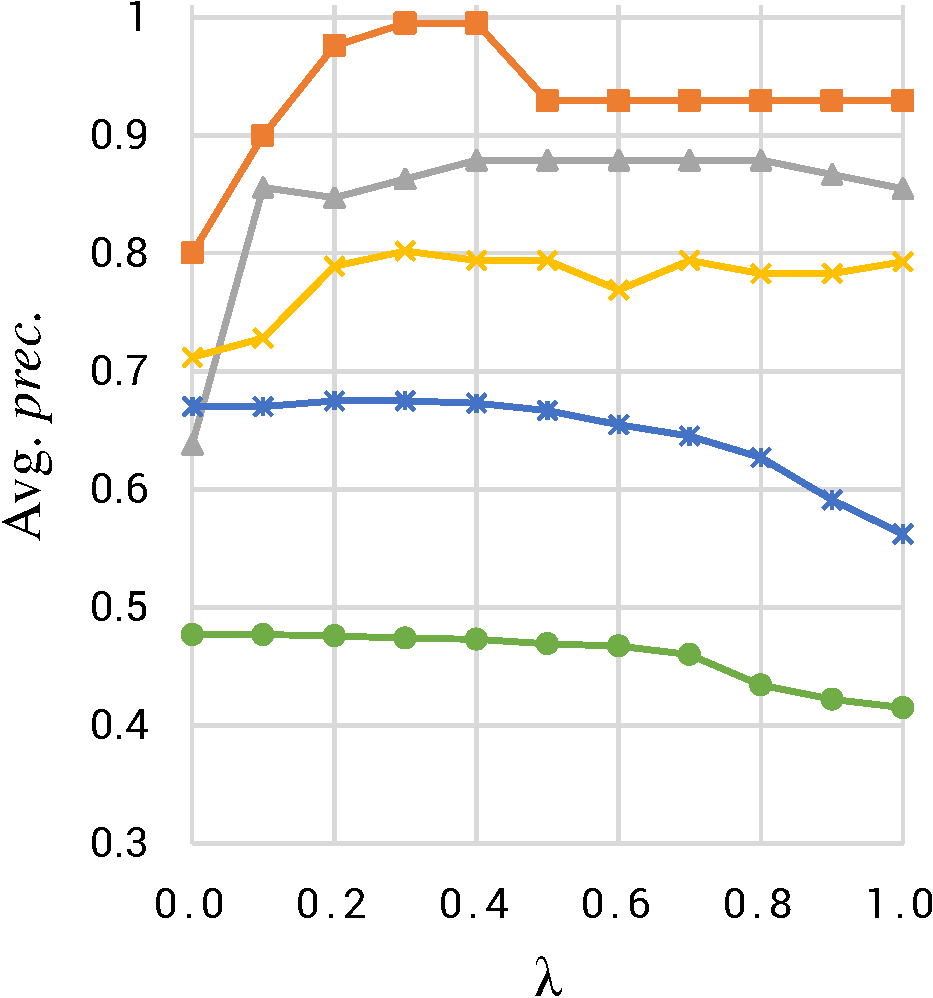
\includegraphics[width=0.33\textwidth]{figures/new_exp1/wiki44k_transe_conf-crop.pdf} }}
%    \subfloat[Wiki44K(conf + SSP)]{{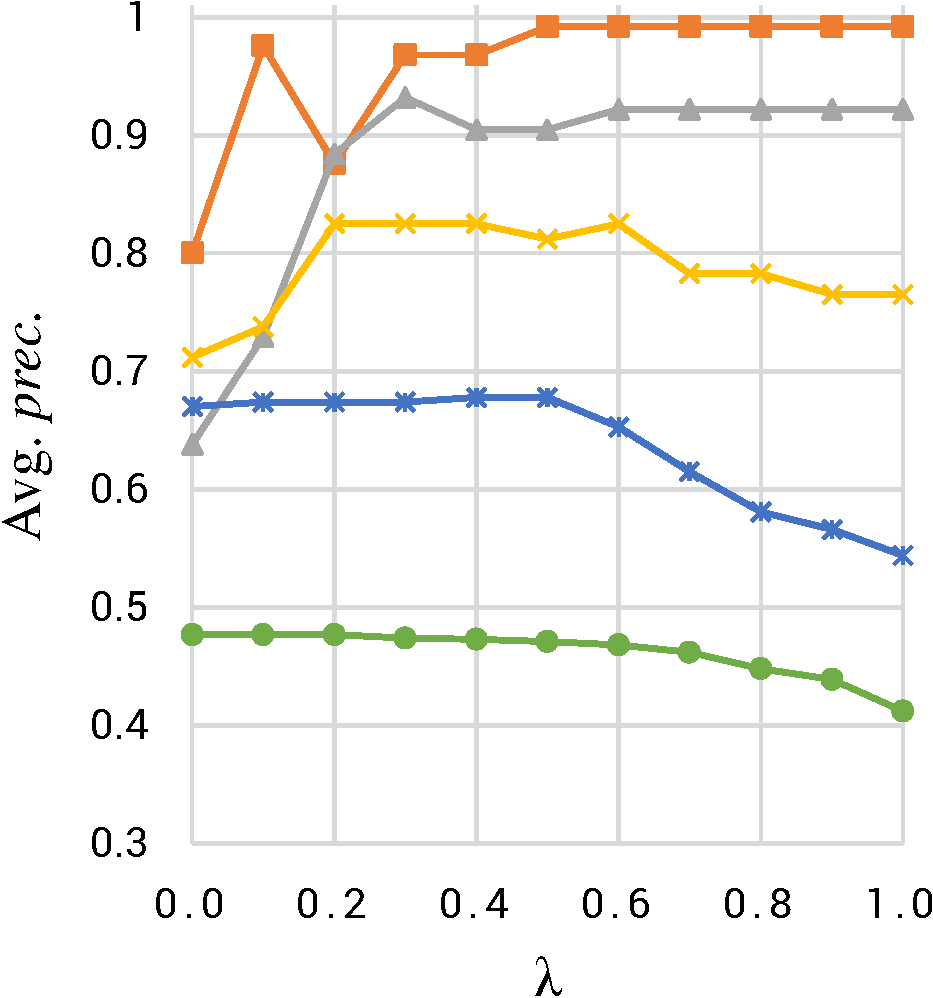
\includegraphics[width=0.33\textwidth]{figures/new_exp1/wiki44k_ssp_conf-crop.pdf} }}
%    % \subfloat[PCA Confidence + TransE]{{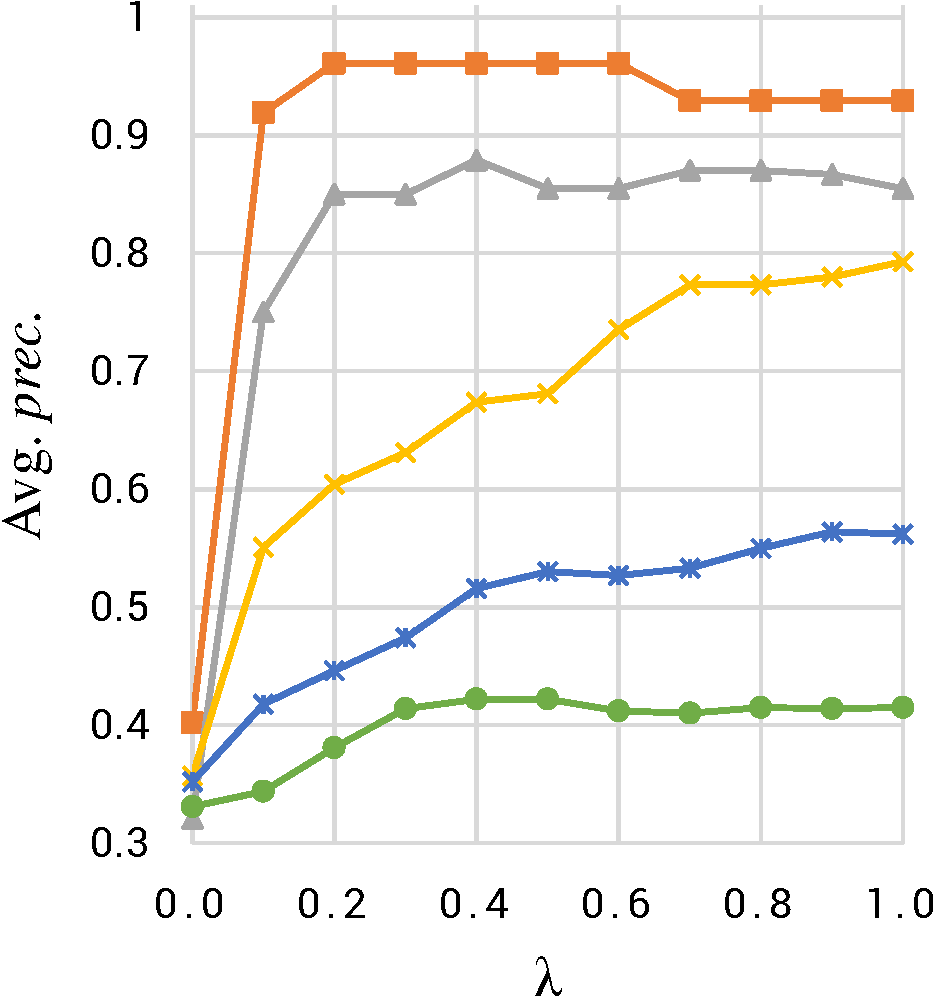
\includegraphics[width=0.5\textwidth]{figures/new_exp1/wiki44k_transe_pca-crop.pdf} }}
%    \subfloat[Wiki44K(pcaconf + SSP)]{{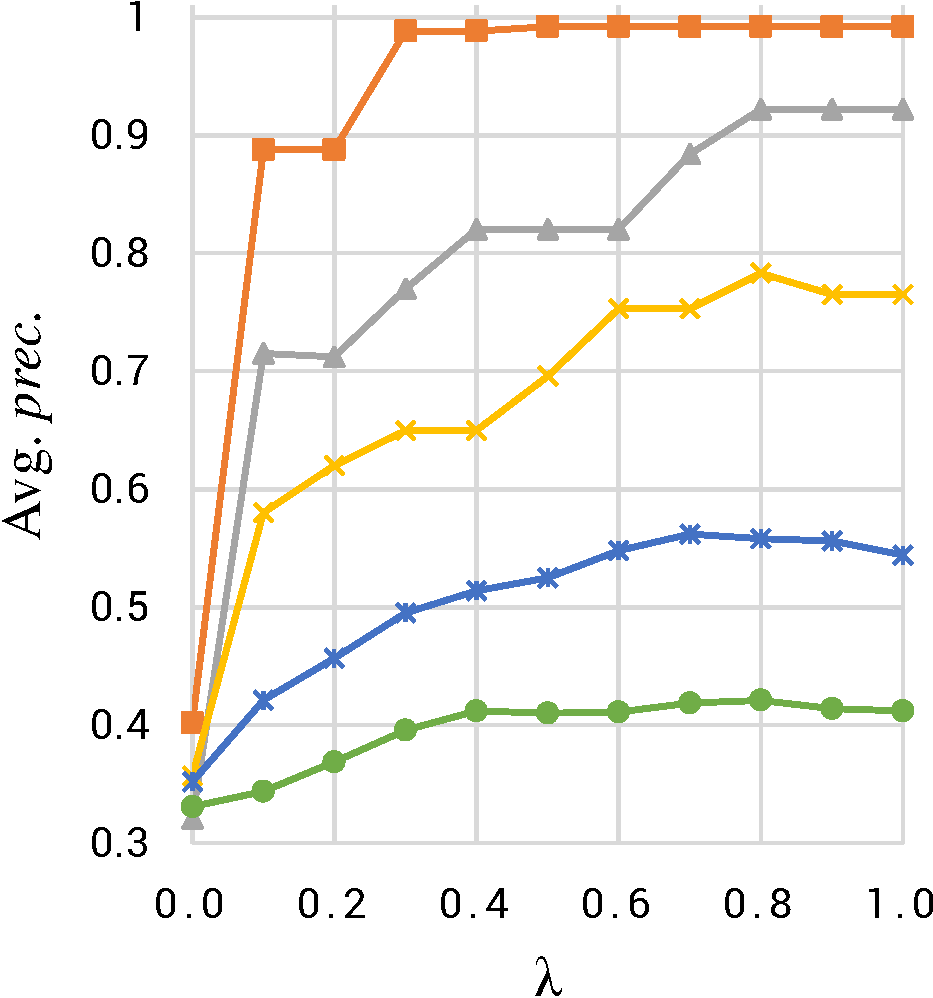
\includegraphics[width=0.33\textwidth]{figures/new_exp1/wiki44k_ssp_pca-crop.pdf} }}\\
%    
%    \caption{Avg. \textit{predictions precision} of the top rules with various \textit{embedding weights} \gad{figures labels should be updated and height should be reduced }}
%    \label{fig:fb15k_and_wiki44k}
%\end{figure}
In this experiment we study the effect of using our hybrid embedding-based 
rule measure $\mu$ from Equation~\ref{eq:hm} on the 
rule ranking compared to traditional measures \add{and embedding models independently. }
We do it by first 
learning rules of the form $r:\;h(X,Z) \leftarrow p(X,Y), q(Y,Z)$ from $\cG$ where $\mi{\textit{r-supp}(r,\cG)\geq 10}$, $\mi{conf(r,\cG)\in [0.1,1)}$ and $\mi{\textit{h-cover}(r,\cG)\geq 0.01}$. 
Then, we rank these rules using Equation~\ref{eq:hm} with $\lambda\in \{0, 0.1, 0.2, \dotsc, 1\}$, $\mu_1\in \{\mi{conf,conf_{pca}}\}$ and with $\mu_2$ that is computed by relying on TransE, HolE and SSP.
\dl{Note that $\lambda=0$ corresponds to the standard rule measure $\mu_1$ alone.}
\add{Note that $\lambda=0$ simulates learning rules using the standard measure $\mu_1$ similar to~\cite{amie}, while $\lambda=1$ corresponds to ranking rules solely based on the predictions of the embedding models. Configuring $\lambda$ indirectly allows us to compare our hybrid measure to both traditional measures and quality of embedding models.}

Figure~\ref{fig:diff_lambda} shows the 
average prediction precision $pred\_prec_{CW}$ of the \textit{top-k} rules ranked using our measure $\mu$ for different embedding weights $\lambda$ (\textit{x-axis}). 
In particular, in Figures~\ref{fig:fb-HoLE-Conf},~\ref{fig:fb-SSP-Conf},~\ref{fig:wi-TransE-Conf}, and~\ref{fig:wi-SSP-Conf} 
we observe that combining confidence with any 
embedding model increases the average prediction precision for $0\leq \lambda\leq 0.3$. 
Moreover, we observe the decrease of prediction precision for $0.4 \leq \lambda\leq 1$ and \textit{top-k} rules learned from FB15K when $k\geq 20$ and from Wiki44K when $k\geq 10$. 
This 
shows that the combination of $\mu_1$ and $\mu_2$ gives noticeable positive effect 
on the prediction results. \add{Ranking using hybrid measure with $\lambda$ around 0.3 achieves better results than both the traditional rule learning and embedding models.} On the other hand, for $\mu_1=\mi{conf_{pca}}$ the precision increases significantly when combined with embedding models and only decreases slightly 
for $\lambda=1$ (Figures~\ref{fig:fb-SSP-PCA},\ref{fig:wi-SSP-PCA}). 
Utilizing $\mi{conf_{pca}}$ instead of $\mi{conf}$ as $\mu_1$ in our hybrid measure is less effective, since 
our training data $\cG$ is randomly sampled 
breaking the 
partial completeness assumption adopted by the PCA confidence. 

\begin{table}[t]
\scriptsize
%\tiny
\centering
\begin{tabular}{c |r r r r |r r r r} 
 \multirow{3}{*}{\textbf{\textit{top-k}}} & \multicolumn{4}{c}{\textbf{FB15K}} & \multicolumn{4}{|c}{\textbf{Wiki44K}} \\
 \cmidrule{2-9}
 & \textbf{{~~}Conf}&  \textbf{{~~~~~~~~}PCA} & \textbf{Conf-HolE}& \textbf{Conf-SSP} &  \textbf{{~~}Conf}&  \textbf{{~~~~~~~~}PCA} & \textbf{Conf-TransE}& \textbf{Conf-SSP}\\
  & {\scriptsize($\lambda=0$)}  & {\scriptsize($\lambda=0$)} & {\scriptsize($\lambda=0.3$)} & {\scriptsize($\lambda=0.3$)} & {\scriptsize($\lambda=0$)} & {\scriptsize($\lambda=0$)} &{\scriptsize($\lambda=0.3$)} & {\scriptsize($\lambda=0.3$)}\\
 \midrule
 \textbf{5} & 0.800 & 0.638 & \textbf{1.000} & \textbf{1.000} & 0.800 & 0.402 & \textbf{0.995} & 0.968\\
\textbf{10} & 0.900 & 0.506 & \textbf{1.000} & \textbf{1.000} & 0.638 & 0.321 & 0.863 & \textbf{0.932} \\
\textbf{20} & 0.900 & 0.499 & 0.950 & \textbf{1.000} & 0.712 & 0.357 & 0.802 & \textbf{0.825}\\
\textbf{50} & 0.881 & 0.410 & 0.936 & \textbf{0.937} & 0.670 & 0.352 & \textbf{0.675} & 0.674 \\
\textbf{100} & 0.855 & 0.348 & 0.885 & \textbf{0.895} & \textbf{0.477} & 0.331 & 0.474 & 0.474\\
\textbf{200} & 0.842 & 0.355 & 0.870 & \textbf{0.875} & -- & -- & -- & -- \\
 \bottomrule
\end{tabular}
\caption{$pred\_prec_{CW}$ of the \textit{top-k} rules learned using different measures.}
\label{table:avg_quality}
\vspace*{-3mm}
\end{table}


Table~\ref{table:avg_quality} compactly summarizes the average prediction precision of \textit{top-k} rules ranked by
the standard rule measures and our $\mu$ for the best value of $\lambda=0.3$ and highlights the effect of using the better embedding model (text-enhanced vs standard).
We observe that the accuracy of a utilized embedding model is naturally propagated to the accuracy of the rules that we obtain using our hybrid ranking measure $\mu$. This demonstrates that the use of a better embedding model positively effects 
the quality of learned rules. 


\subsection{Horn Rule Learning}
\label{sec:RuLES_vs_AMIE}

\begin{table}[t]
\scriptsize
\centering
\begin{tabular}{c|r r|r r|r r|r r|r r|r r}

 \multirow{3}{*}{\textbf{\textit{top-k}}}&\multicolumn{6}{|c}{\textbf{FB15K}} & \multicolumn{6}{|c}{\textbf{Wiki44K}}\\
 \cmidrule{2-13}&\multicolumn{2}{|c}{\textbf{AMIE-PCA}}&\multicolumn{2}{|c|}{\textbf{AMIE-Conf}}&\multicolumn{2}{|c}{\textbf{RuLES}}&\multicolumn{2}{|c}{\textbf{AMIE-PCA}}&\multicolumn{2}{|c}{\textbf{AMIE-Conf}}&\multicolumn{2}{|c}{\textbf{RuLES}} \\
 & \textit{Facts} & \textit{Prec.} & \textit{Facts} & \textit{Prec.} & \textit{Facts} & \textit{Prec.} &\textit{Facts} & \textit{Prec.} &\textit{Facts} & \textit{Prec.} &\textit{Facts} & \textit{Prec.} \\
 \midrule
 \textbf{20} & 1029 & 0.28 & 82 & 0.63 & 44 & 1.00 & 185 & 0.73 & 91 & 0.95 & 3291 & 0.98\\
 \textbf{50} & 1716 & 0.43 & 190 & 0.74 & 186 & 0.92 & 47099 & 0.10 & 3594 & 0.95 & 6154 & 0.88 \\
\textbf{100} & 3085 & 0.65 & 255 & 0.78 & 539 & 0.80 & 56831 & 0.20 & 13870 & 0.83 & 13253 & 0.82 \\
\textbf{200} & 10586 & 0.62 & 1210 & 0.83 & 1205 & 0.88 & 82288 & 0.39 & 19538 & 0.72 & 20408 & 0.73 \\
\textbf{500} & 40050 & 0.51 & 2702 & 0.75 & 7124 & 0.95 & 219264 & 0.35 & 124836 & 0.23 & 128256 & 0.48 \\
 \bottomrule
\end{tabular}
\caption{$pred\_prec_{OW}$ of the \textit{top-k} rules generated by RuLES and AMIE.}
\label{table:amie_vs_RuLES}
\vspace*{-3mm}
\end{table}

\begin{table}[t]
\scriptsize
\centering
\begin{tabular}{c|r r|r r}

 \multirow{2}{*}{}&\multicolumn{2}{c}{\textbf{Family-NeuralLP}}&\multicolumn{2}{|c}{\textbf{Family-Conf-TransE}}\\
\textbf{\emph{top-k}}& \textit{Facts} & \textit{Prec.} & \textit{Facts} & \textit{Prec.} \\
 \midrule
\textbf{10} & 3709 & 0.72 & 4201 & 0.68 \\
\textbf{20} & 8821 & 0.53 & 6957 & 0.72 \\
\textbf{30} & 11337 & 0.49 & 9368 & 0.71 \\
\textbf{40} & 14662 & 0.46 & 11502 & 0.72 \\
\textbf{50} & 18768 & 0.40 & 14547 & 0.62 \\
 \bottomrule
\end{tabular}
\caption{$pred\_prec_{OW}$ of the \textit{top-k} rules generated by NeuralLP and RuLES.}
\label{table:neurallp_vs_rules}
%\thi{This is added to compare NeuralLP and RuLES}
\vspace*{-3mm}
\end{table}


In this experiment, we compare RuLES under Conf-SSP configuration (with embedding weight $\lambda = 0.3$) with the state-of-art Horn rule learning system AMIE. We used the default AMIE-PCA configuration with $\mi{conf_{pca}}$ and 
AMIE-Conf with $\mi{conf}$ measures respectively. For a fair comparison, we set the two configurations of AMIE and our system  to generate rules with at most three positive atoms and filtered them based on minimum confidence of $0.1$, head coverage of $0.01$ and rule support of $10$ in case of FB15K and $2$ in case of Wiki44K. We then filtered out all rules with $\mi{conf(r,\cG) = 1}$, as they 
do not produce any predictions.

Table~\ref{table:amie_vs_RuLES} shows the number of facts (see the \textit{Facts} column) predicted by 
the set $R$ of \textit{top-k} rules 
in the described settings 
and their prediction precision $pred\_prec_{OW}(R)$ (see the \textit{Prec.} column). 
The size of the random sample 
outside $\cG^i_{appr}$ is 20. 
We can observe that on FB15K, RuLES consistently outperforms both AMIE configurations. The \textit{top-20} rules have the highest precision difference (outperforming AMIE-PCA and AMIE-Conf by $72\%$ and $37\%$ respectively).
This is explained by the fact that the hybrid embedding quality penalizes rules with higher number of false predictions. 
For Wiki44K, RuLES is capable of achieving better precision in most of the cases. 
Notably, for the \textit{top-20} rules RuLES predicted significantly more facts then competitors yet with a high precision. 

In table~\ref{table:neurallp_vs_rules}, we compare RuLES with the recently developed NeuralLP system~\cite{DBLP:conf/nips/YangYC17}. For this we 
utilized the Family dataset used by NeuralLP 
with 28K facts over 3K entities and 12 relations. 
Starting from the \textit{top-20} rules RuLES is capable of achieving significantly better precision. For the \textit{top-10} rules the precision of NeuralLP is slightly better, but RuLES predicts many more facts.


\subsection{RuLES for Exception-Aware Rule Learning}
%----------------------------------------------------------------%
In this experiment, we aim at evaluating the effectiveness of RuLES 
for learning exception-aware rules.
First, consider in Table~\ref{figure:examples} examples of such rules learned by RuLES over Wiki44K dataset. 
 The first rule $r^1$ says that a person is a citizen of the country where his alma mater is located, unless it is a research institution, 
since most 
researchers in universities are foreigners. The second rule $r^2$ states that the scriptwriter of some artistic work is also the scriptwriter of its sequel unless it is a TV series, which actually reflects the common practice of having several screenwriters for different seasons. Additionally, $r^3$ encodes that someone belonged to a 
noble family if his/her 
spouse is also from the same noble family, excluding the Chinese dynasties. 

To quantify the quality of RuLES in learning non-monotonic rules, we compare the Conf-SSP configuration of RuLES (with embedding weight $\lambda = 0.3$) with RUMIS~\cite{trantowards}, which is a revision-based 
non-monotonic rule 
learning system, which 
extracts rules 
of the form  
$\mi{r:\;h(X,Z) \leftarrow p(X,Y), q(Y,Z), not\; E}$, where $E$ is either $e(X,Z)$ or 
$e(X)$.
For a fair comparison we restricted RuLES to learn rules of the same form.   
We configured both systems 
setting the minimum rule support threshold to 
$10$ and exception confidence for RuLES to $0.05$. 
To enable the systems to 
learn rules with exceptions of the form 
$e(X)$, we enriched 
our KGs with \textit{types} 
from original Freebase and Wikidata KGs. 

%!TEX root = ../main.tex


\begin{table}[t]
\centering
\footnotesize
\begin{tabular}{|cl|}
	\hline
	%$r_1:$ & $has\_family(X, Y) \leftarrow has\_child(Z, X), has\_family(Z, Y), \textbf{not}\ has\_mother(X, Z).$\\
$r^1{:}$ & $\mi{nationality(X{,}\, Y)}\, {\leftarrow}\, \mi{graduated\_from(X{,}\, Z)}{,}\, \mi{in\_country(Z{,}\, Y)},
	\textbf{not}\ \mi{research\_uni(Z)}$\\
$r^2{:}$ & $\mi{scriptwriter\_of}(X{,}\, Y)\, {\leftarrow}\, \mi{preceded\_by(X{,}\, Z)}{,}\, \mi{scriptwriter\_of(Z{,}\, Y)},
\textbf{not}\ \mi{tv\_series(Z)}$\\
$r^3{:}$ &$\mi{noble\_family(X{,}\, Y)}\, {\leftarrow}\, \mi{ spouse(X{,}\, Z)}{,}\, \mi{noble\_family(Z{,}\, Y)}{,}\,  \textbf{not}\ \mi{ chinese\_dynasties(Y)}$\\
%$r_3:$ &$\mi{sister(X, Y)} \leftarrow \mi{sister(Y, X)}, \textbf{not}\ \mi{brother(X, Y)}$\\

	\hline
\end{tabular}
\caption{Example rules with exception generated by RuLES.}
\vspace*{-3mm}
\label{figure:examples}
\end{table}

%!TEX root = ../main.tex

% \begin{table}[t]
% \centering
% \begin{tabular}{|r|r r|r r|r r|r r|}
%  \hline
%  \multirow{3}{*}{$top-k$}&\multicolumn{4}{|c|}{FB15K} & \multicolumn{4}{|c|}{WIKI44K}\\
%  \cline{2-9}&\multicolumn{2}{|c|}{RUMIS}&\multicolumn{2}{|c|}{RuLES}&\multicolumn{2}{|c|}{RUMIS}&\multicolumn{2}{|c|}{RuLES} \\
%  & $Avg.scr.$ & $Avg.inc.$ & $Avg.scr.$ & $Avg.inc.$& $Avg.scr.$ & $Avg.inc.$& $Avg.scr.$ & $Avg.inc.$ \\
%  \hline
%  20 & 0.791 & 0.024 & 1.000 & 0.047 & 0.743 & 0.067 & 0.803 & 0.024 \\
%  50 & 0.826 & 0.015 & 1.000 & 0.045 & 0.609 & 0.054 & 0.701 & 0.026 \\
% 100 & 0.859 & 0.026 & 0.990 & 0.047 & 0.417 & 0.033 & 0.539 & 0.011 \\
% 200 & 0.848 & 0.034 & 0.977 & 0.065 & 0.253 & 0.022 & 0.339 & 0.017 \\
% 500 & 0.745 & 0.043 & 0.958 & 0.079 & -- & -- & -- & -- \\
% \hline
% \end{tabular}
% \caption{Average prediction score of some top non-monotonic rules from RuLES vs RUMIS.}
% \label{table:exception_prediction_result}
% \vspace*{-3mm}
% \end{table}

%\begin{table}[t]
%\centering
%\begin{tabular}{|c|r r|r r|r r|r r|}
% \hline
% \multirow{3}{*}{\textbf{\textit{top-k}}}&\multicolumn{4}{|c|}{\textbf{FB15K}} & \multicolumn{4}{|c|}{\textbf{Wiki44K}}\\
% \cline{2-9}&\multicolumn{2}{|c|}{\textbf{RUMIS}}&\multicolumn{2}{|c|}{\textbf{RuLES}}&\multicolumn{2}{|c|}{\textbf{RUMIS}}&\multicolumn{2}{|c|}{\textbf{RuLES}} \\
% & $Facts$ & $Prec.$ & $Facts$ & $Prec.$& $Facts$ & $Prec.$& $Facts$ & $Prec.$ \\
% \hline
%\textbf{20} & 672 & 0.95 & 34 & 0.97 & 5844 & 0.93 & 5640 & 0.93 \\
%\textbf{50} & 1797 & 0.94 & 158 & 0.99 & 8585 & 0.83 & 13333 & 0.84 \\
%\textbf{100} & 2672 & 0.94 & 434 & 0.99 & 21081 & 0.76 & 25265 & 0.81 \\
%\textbf{200} & 4103 & 0.87 & 1155 & 0.96 & 50957 & 0.51 & 43677 & 0.67 \\
%\textbf{500} & 13439 & 0.76 & 5466 & 0.90 & -- & -- & -- & -- \\
%\hline
%\end{tabular}
%\caption{$pred\_prec_{OW}$ of the \textit{top-k} rules learned by RUMIS and RuLES.}
%\label{table:exception_prediction_result}
%\vspace*{-3mm}
%\end{table}

\begin{table}[t]
\scriptsize
\centering
\begin{tabular}{r | r r| r r | r r |r r}
 & \multicolumn{4}{c}{\textbf{FB15K}} & \multicolumn{4}{|c}{\textbf{Wiki44K}} \\
 \cmidrule{2-9}&\multicolumn{2}{c}{\textbf{RUMIS}}&\multicolumn{2}{|c}{\textbf{RuLES}}&\multicolumn{2}{|c}{\textbf{RUMIS}}&\multicolumn{2}{|c}{\textbf{RuLES}} \\
\textbf{\textit{top-k}} & \emph{Facts} & \emph{Prec.} & \emph{Facts} & \emph{Prec.} & \emph{Facts} & \emph{Prec.}& \emph{Facts} & \emph{Prec.} \\
 \midrule
\textbf{20} & 672 & 0.95 & 34 & 0.97 & 5844 & 0.93 & 5640 & 0.93 \\
\textbf{50} & 1797 & 0.94 & 158 & 0.99 & 8585 & 0.83 & 13333 & 0.84 \\
\textbf{100} & 2672 & 0.94 & 434 & 0.99 & 21081 & 0.76 & 25265 & 0.81 \\
\textbf{200} & 4103 & 0.87 & 1155 & 0.96 & 50957 & 0.51 & 43677 & 0.67 \\
\textbf{500} & 13439 & 0.76 & 5466 & 0.90 & -- & -- & -- & -- \\
\bottomrule
\end{tabular}
%
\qquad
%
\begin{tabular}{r | r r| r r | r r |r r}
 & \multicolumn{4}{c}{\textbf{FB15K}} & \multicolumn{4}{|c}{\textbf{Wiki44K}} \\
 \cmidrule{2-9}&\multicolumn{2}{c}{\textbf{RUMIS}}&\multicolumn{2}{|c}{\textbf{RuLES}}&\multicolumn{2}{|c}{\textbf{RUMIS}}&\multicolumn{2}{|c}{\textbf{RuLES}} \\
\textbf{\textit{top-k}} & \emph{Facts} & \emph{Prec.} & \emph{Facts} & \emph{Prec.} & \emph{Facts} & \emph{Prec.}& \emph{Facts} & \emph{Prec.} \\
 \midrule
\textbf{20} & 76 & 0.70 & 111 & 0.68 & 63 & 0.47 & 81 & 0.94 \\
\textbf{50} & 126 & 0.51 & 435 & 0.74 & 191 & 0.28 & 611 & 0.69 \\
\textbf{100} & 183 & 0.43 & 680 & 0.76 & 543 & 0.49 & 1698 & 0.79 \\
\textbf{200} & 310 & 0.30 & 1112 & 0.87 & 4861 & 0.40 & 3175 & 0.80 \\
\textbf{500} & 1155 & 0.53 & 3760 & 0.59 & -- & -- & -- & -- \\
\bottomrule
\end{tabular}

\caption{$pred\_prec_{OW}$ (left) and $rev\_prec_{OW}$ (right)
of the \textit{top-k} rules learned by RUMIS and RuLES.}
\label{table:exception_prediction_result}
\vspace*{-3mm}
\end{table}



Table~\ref{table:exception_prediction_result} (left) reports the number of predictions produced by a rule set $R$ of 
\textit{top-k} non-monotonic rules learned 
by both systems as well as 
their precision $pred\_prec_{OW}(R)$ with a sample of 20 prediction outside $\cG^i_{appr}$. The results show that RuLES consistently outperforms RUMIS 
on both datasets. For Wiki44K, and $k\in\{50,100\}$, the \textit{top-k} rules produced by RuLES predicted more facts than those induced by the competitor 
achieving higher overall precision. 
Regarding the number of predictions, the converse holds for the FB15K KG; however, the rules learned by RuLES are still more accurate.

To evaluate the quality of the chosen exceptions, we compare the $rev\_prec_{OW}(R)$ with a sample of 20 predictions. Observe that in Table~\ref{table:exception_prediction_result} (right), rules induced by RuLES prevented the generation of more facts than RUMIS. 
In all of the cases apart from \textit{top-20} for FB15K, our system 
managed to remove a larger fraction of erroneous predictions. 
For Wiki44K, RuLES consistently performs twice as good as RUMIS. 
In conclusion, the guidance from the embedding model 
exploited in our system 
gives us hints on which among the possible exception candidates likely correspond to noise.   











